\usepackage[utf8]{inputenc}
\usepackage[T1]{fontenc}
\usepackage[ngerman]{babel}
\usepackage{array}
\usepackage{bookmark}
\usepackage{textpos}
\usepackage{wasysym}
%\usepackage{listliketab}
\usepackage[NewCommands,NewParameters]{ragged2e}
\usepackage{tikz}
\usepackage{eurosym}
\usepackage{textpos}
\usepackage{comment}

\usetheme{junghans}

\def\insertauthorindicator{Wer?}% Default is "Who?"
\def\insertinstituteindicator{Von?}% Default is "From?"
\def\insertdateindicator{Wann?}% Default is "When?"
%\def\theDate{\today}
\def\theDate{3. Juni 2014}

%\setbeamertemplate{caption}[numbered]

%%neuer Spaltentyp: linksb"undig + Silbentrennung
\newcolumntype{M}[1]{>{\RaggedRight\hspace{0pt}\arraybackslash}p{#1}}

\author{Marius Spix}

\institute[\raisebox{-4mm}{
\includegraphics[width=1.8cm]{images/JW_Kontur}}]{
\includegraphics[scale=0.3]{images/J_60_Schwarz_Reflex_Blue}}
\title{QM-Cockpit}

%\addtobeamertemplate{frametitle}{}{
%\begin{textblock*}{100mm}(-4.15cm,-.55cm)
%
\includegraphics[scale=.33]{images/Fahne2}\end{textblock*}
%}

\AtBeginSection{\frame{\sectionpage}}
%\AtBeginSubsection{\frame{\subsectionpage}}
\newtranslation[to=ngerman]{Section}{Abschnitt}
\newtranslation[to=ngerman]{Subsection}{Unterabschnitt}

\keywords{Abschlusspr"ufung, Fachinformatiker, SAP, Quali"atsmanagement,
Lager, Warenwirtschaft}
\date{\theDate}

\frenchspacing

\begin{document}

\setcounter{framenumber}{0} 
\begin{frame}
  \maketitle
\end{frame}

\setcounter{figure}{0}

\begin{frame}{"Ubersicht}
  \tableofcontents
\end{frame}

\section{Projektumfeld}

\subsection{Betrieb}
\begin{frame}[<+->]{Junghans Unternehmensgruppe}
			\begin{block}{Fakten}
				\begin{itemize}[<+->]
						\item Versandhandelsgruppe
						\item Hauptsitz in Aachen
						\item ca. 540 Mitarbeiter
						\item vertreten in 6 L"andern
				\end{itemize}
			\end{block}

			\begin{block}{Sortimente}
				\begin{itemize}[<+->]
						\item Junghans Wolle
						\item Pro-Idee
				\end{itemize}
			\end{block}
\end{frame}

\begin{frame}[<+->]{Organisation \& Datenverarbeitung}
			\begin{block}{Die DV}
				\begin{itemize}
						\item 21 Mitarbeiter
						\begin{itemize}
							\item IT-Services
							\item \textbf<6>{Anwendungssysteme}
							\item Betriebsorganisation
						\end{itemize}
				\end{itemize}
			\end{block}
			\pause
			\begin{block}{SAP}
				\begin{itemize}[<+->]
						\item Einf"uhrung: Juli 2011
						\item SAP ECC 6.0
						\item SAP NetWeaver BI 7.1
						\item 3-System-Landschaft
				\end{itemize}
			\end{block}
\end{frame}

\subsection{Prozess Wareneingang}
\begin{frame}{Wareneingang}
 \begin{overlayarea}{\textwidth}{.42\textheight}
 	\only<1>{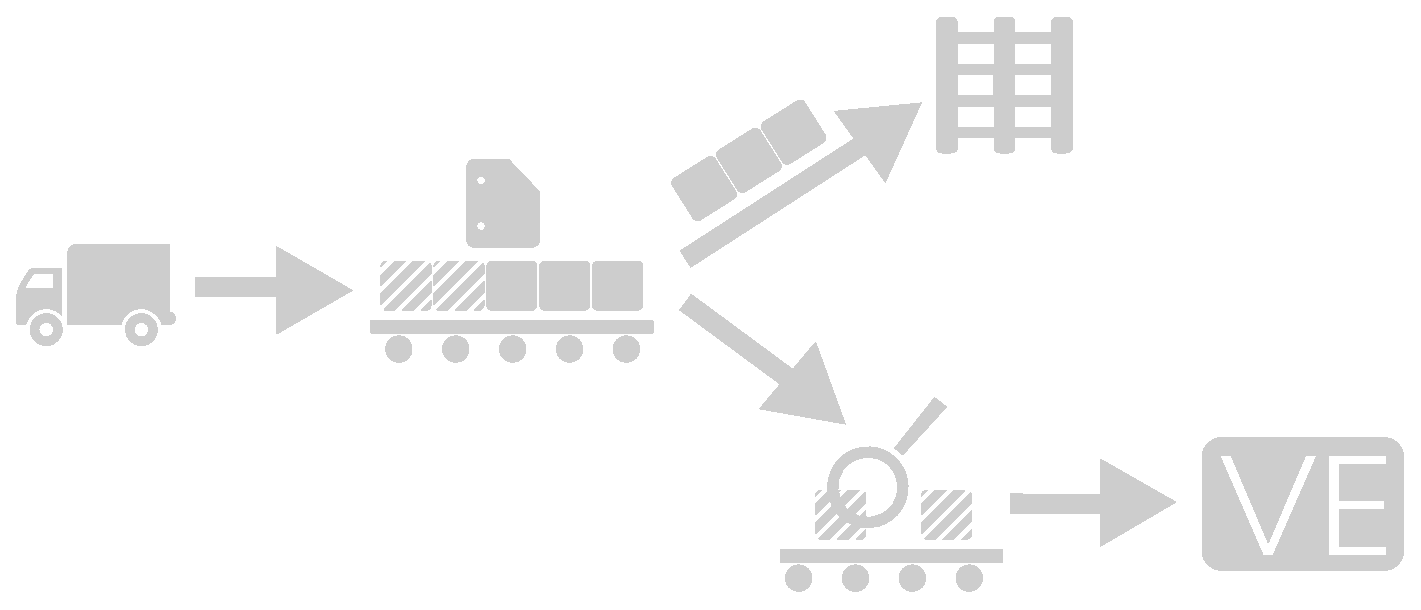
\includegraphics[width=.9\textwidth]{WE0a}<handout:0>}
 	\only<2>{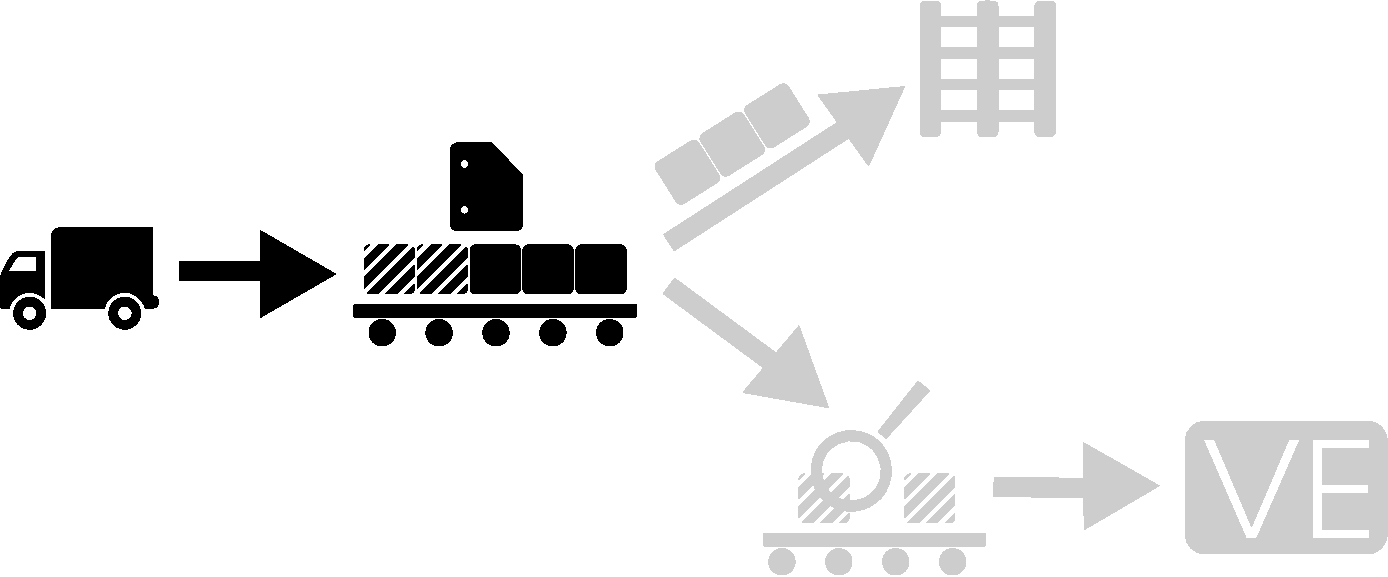
\includegraphics[width=.9\textwidth]{WE1a}<handout:0>}
 	\only<3>{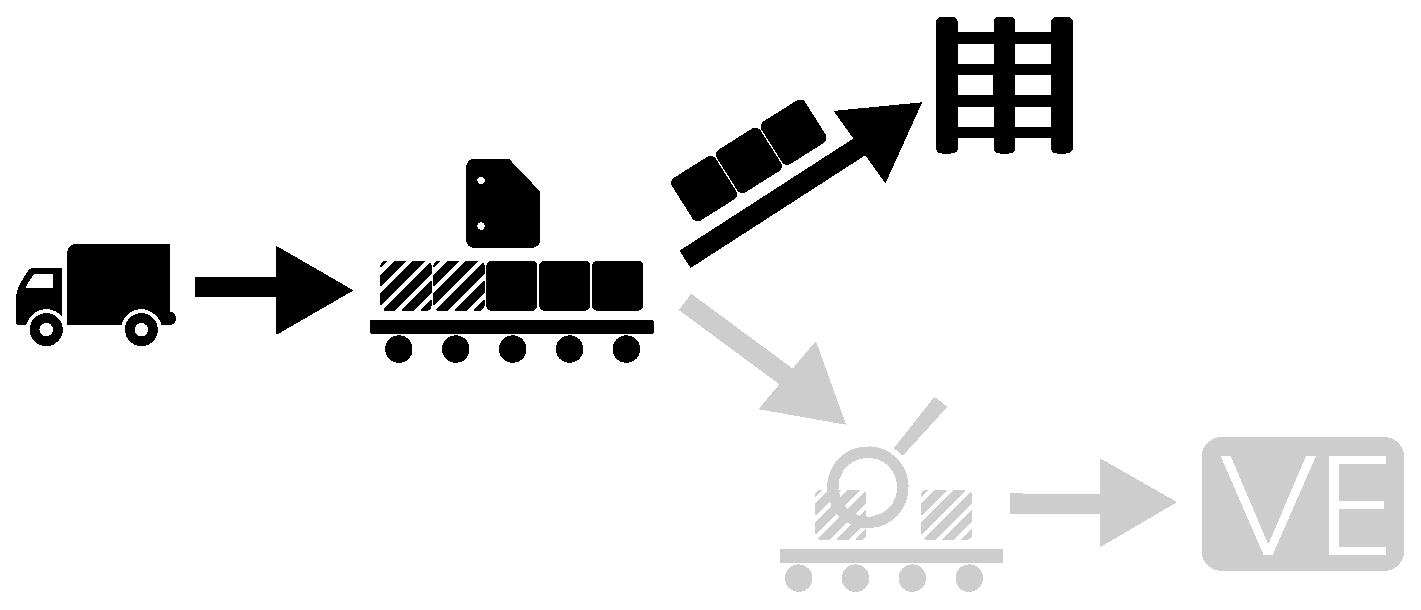
\includegraphics[width=.9\textwidth]{WE2a}<handout:0>}
 	\only<4->{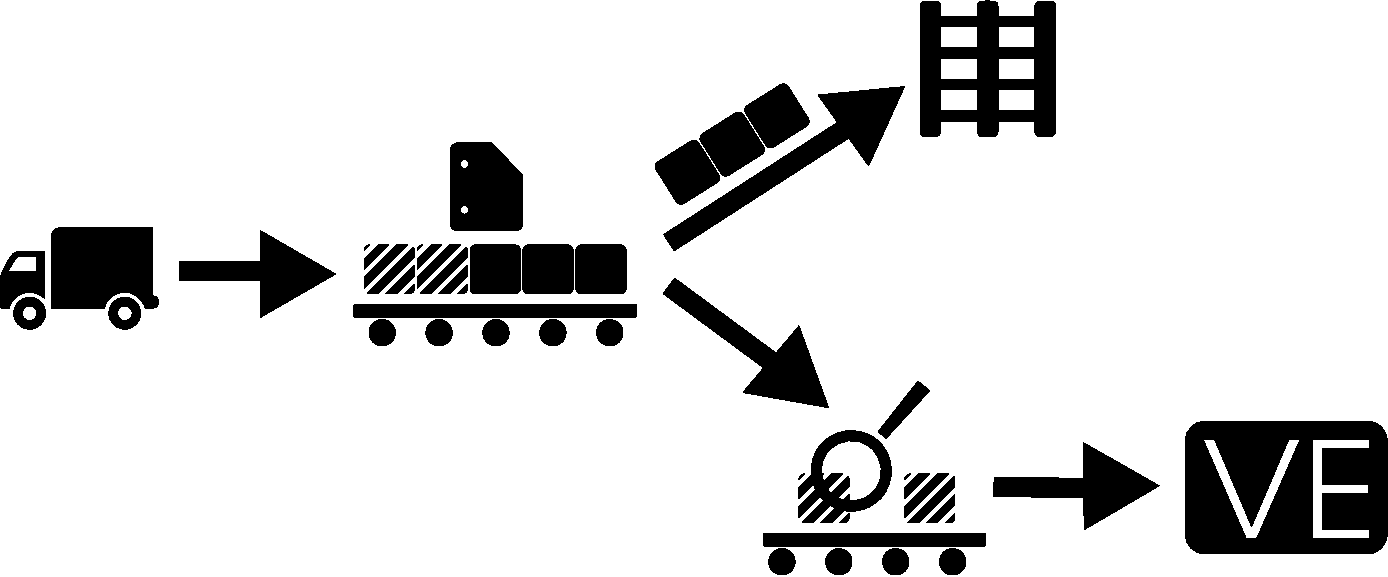
\includegraphics[width=.9\textwidth]{WE3a}}
 \end{overlayarea}
 \begin{overlayarea}{\textwidth}{.58\textheight}
 \only<5->{
 	\vspace{-1ex}
 	\hrulefill
 	\begin{figure}[tbh!]
 	\centering
 	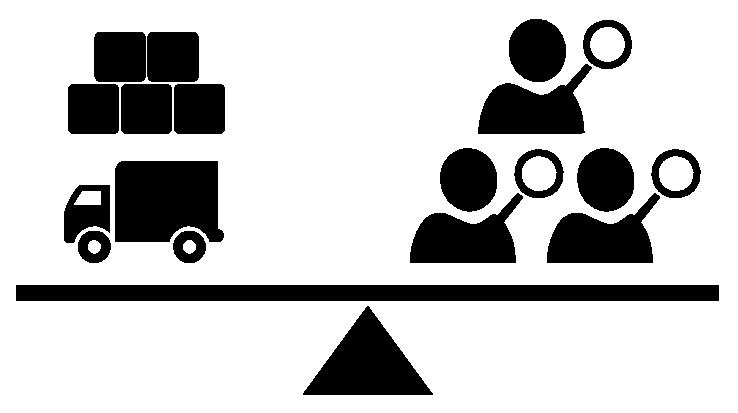
\includegraphics[height=.3\textwidth]{Kapazitaet}
 	\end{figure}
 }
 \end{overlayarea}
\end{frame}

\section{Das Projekt}
\subsection{Ist-Analyse}
\begin{frame}[<+->]{Ist-Analyse}
	\begin{block}{Situation}
		\begin{itemize}[<+->]
			\item Personalplanung: saisonale Schwankungen
			\item{SAP-Einf"uhrung: 2011
			\begin{itemize}
				\item keine Standardfunktionalit"at
				\item diverse Datenquellen
				\item hoher Normalisierungsgrad
			\end{itemize}
			}
			\item Altsystem: Drucklisten
		\end{itemize}
	\end{block}
	\begin{block}{Methoden}
		\begin{itemize}[<+->]
			\item Arbeitsbeobachtung
			\item Interview
			\item Datenbankanalyse
		\end{itemize}
	\end{block}
\end{frame}

\begin{frame}{Derzeitige L"osung}
	\begin{figure}[tbh!]
		
\includegraphics[width=\textwidth]{Strichliste}
	\end{figure}
	\begin{columns}
		\begin{column}{.5\textwidth}
			\begin{figure}[tbh!]
				
\includegraphics[width=.7\textwidth]{Excel}
			\end{figure}
		\end{column}
		\begin{column}{.5\textwidth}
			\begin{figure}[tbh!]
				
\includegraphics[width=.7\textwidth]{Uhr}
			\end{figure}
		\end{column}
	\end{columns}
\end{frame}

\subsection{Soll-Konzept}
\begin{frame}[<+->]{Soll-Konzept}
	\begin{block}{Ziel}
		\begin{itemize}
			\item schnelle Online-Auswertungen
			\item zentrale Controlling-Oberfl"ache
			\item nahtlose Integration ins SAP-Umfeld
			\item Auswertung der Pr"uflosbearbeitungszeit 
		\end{itemize}
	\end{block}
	
	\begin{block}{Herausforderungen}
		\begin{description}[Z"ahlung im ALV Grid]
			\item[Performance]{denormalisiertes Datenmodell}
			\item[Erweiterbarkeit]{Steuertabelle + Factory}
			\item[Z"ahlung im ALV Grid]{Hilfsspalte zum Kumulieren}
		\end{description}
	\end{block}
\end{frame}

\subsection{Durchf"uhrung}
\begin{frame}{Entwicklungsprozess}
 \vspace{2ex}
 \begin{overlayarea}{\textwidth}{\textheight}
  \only<1>{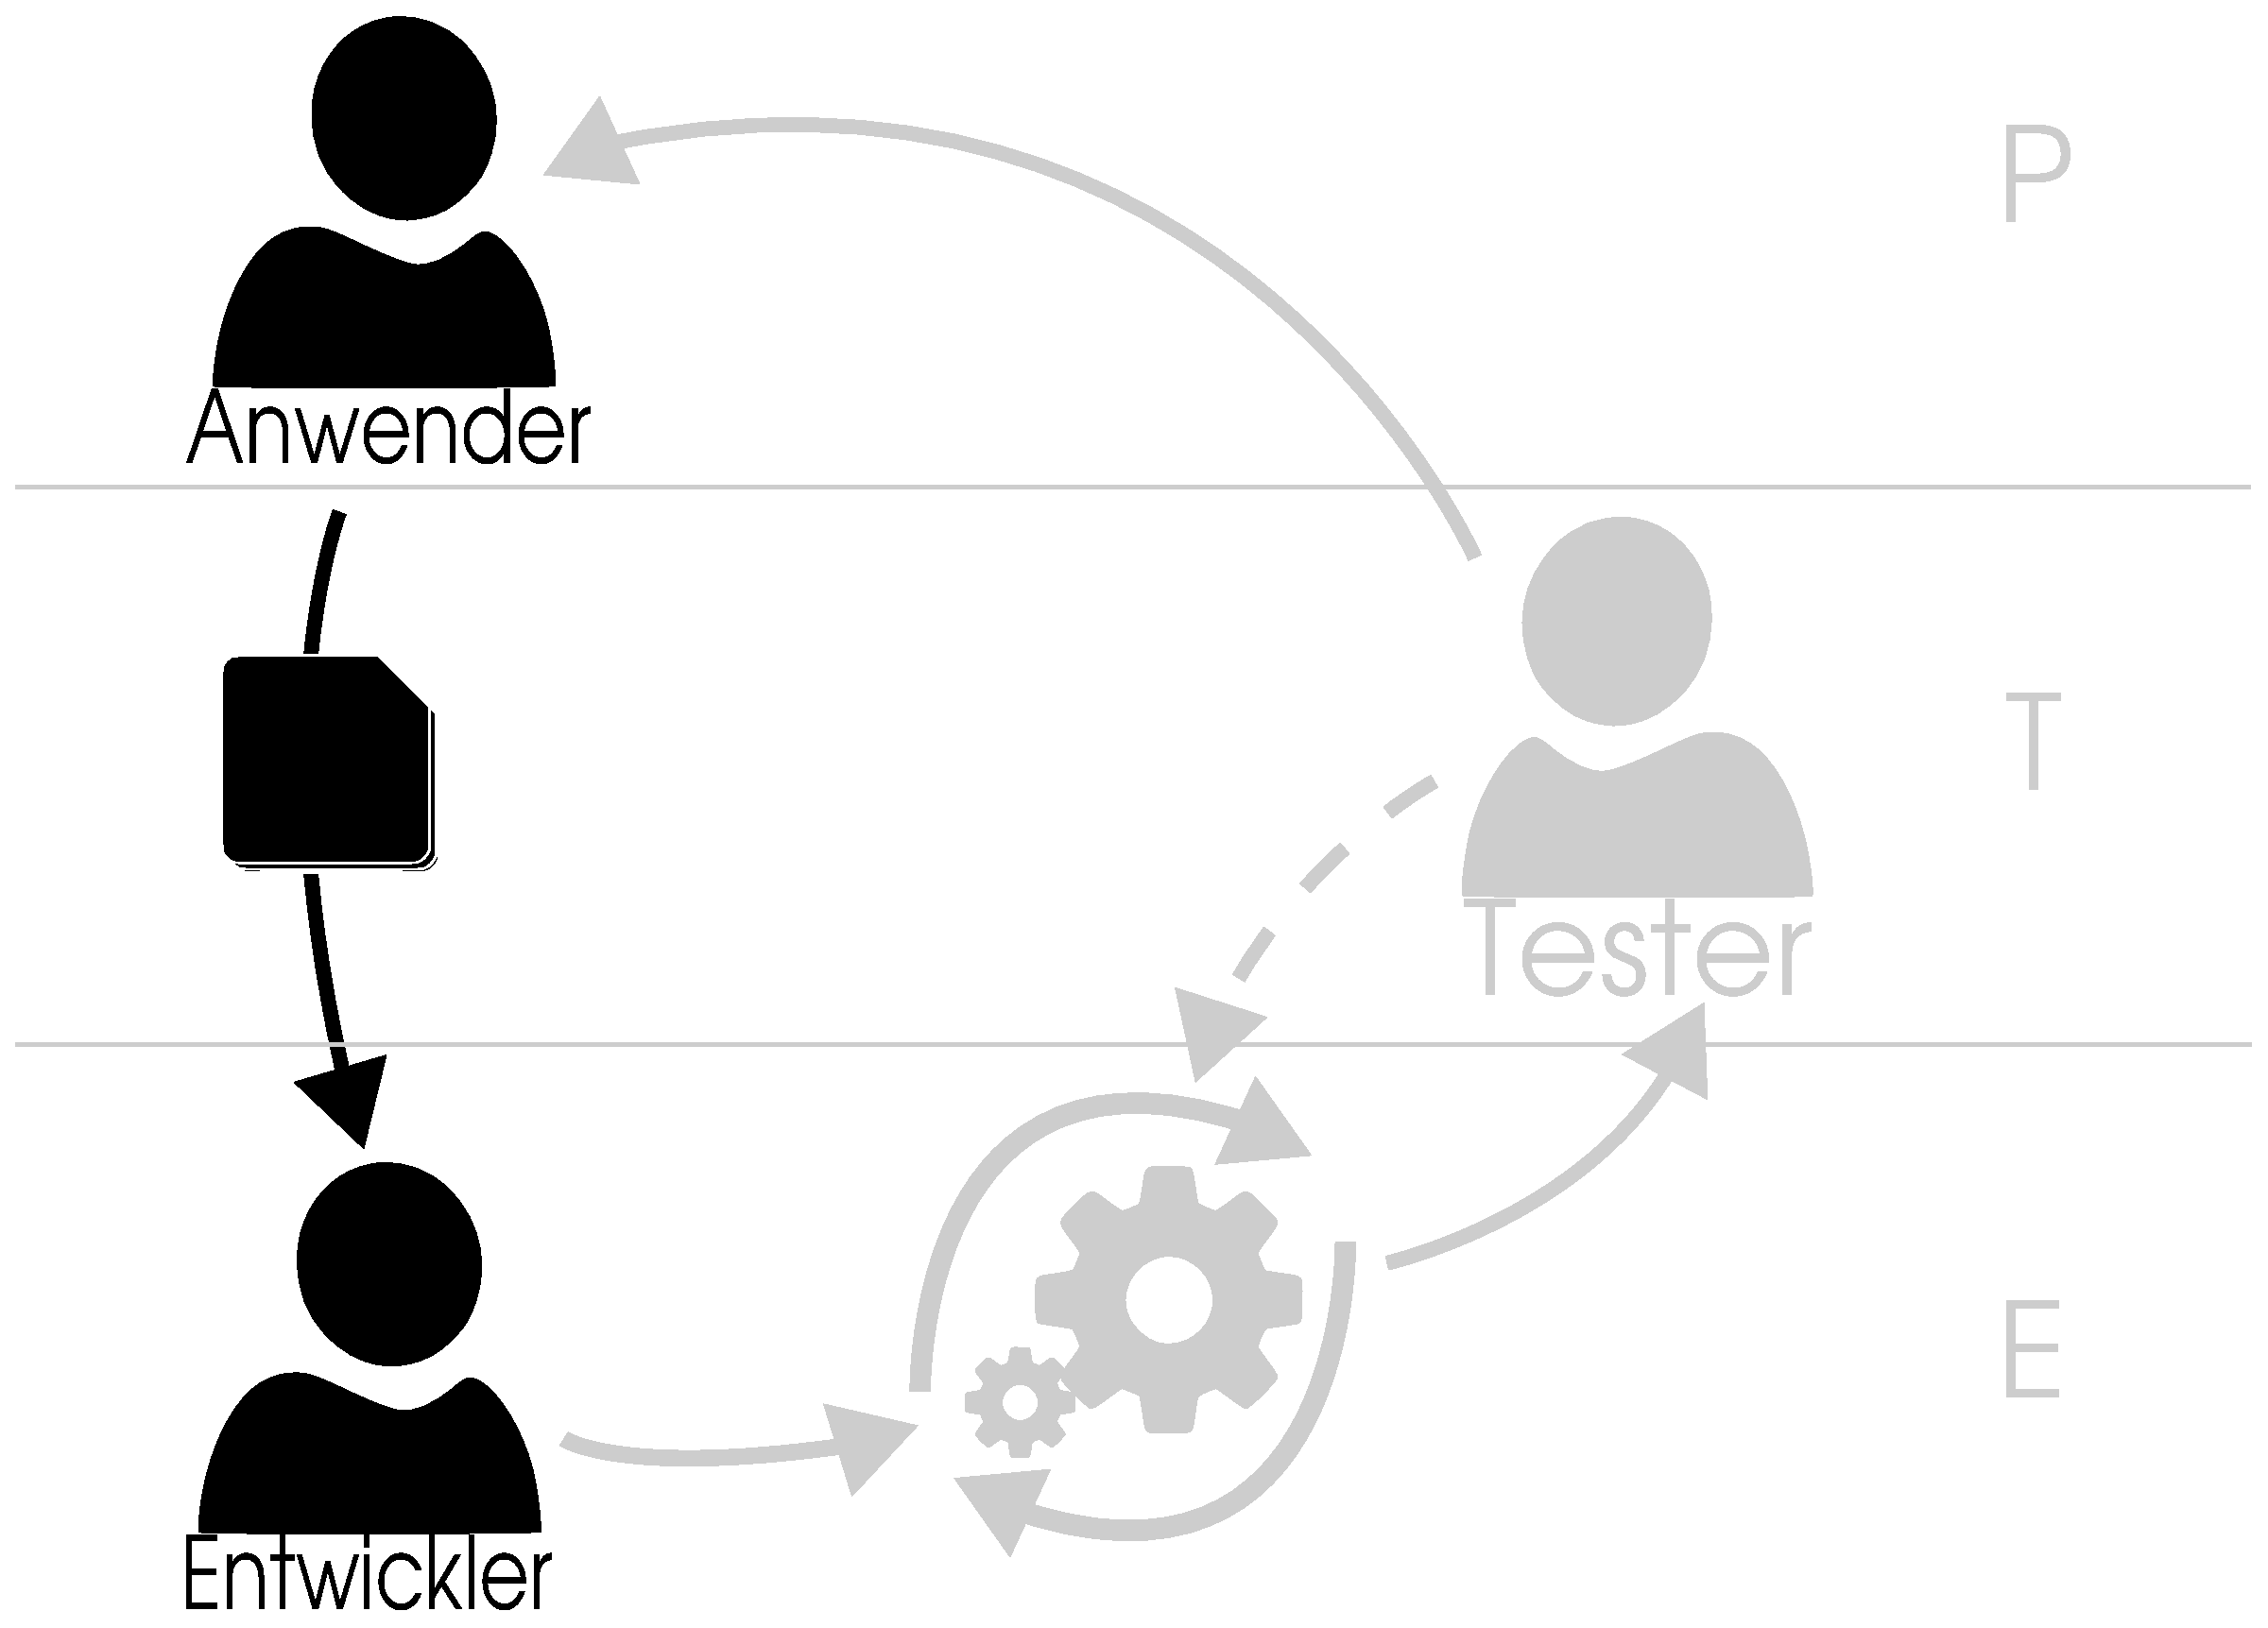
\includegraphics[width=\textwidth]{FDD1}<handout:0>}
  \only<2>{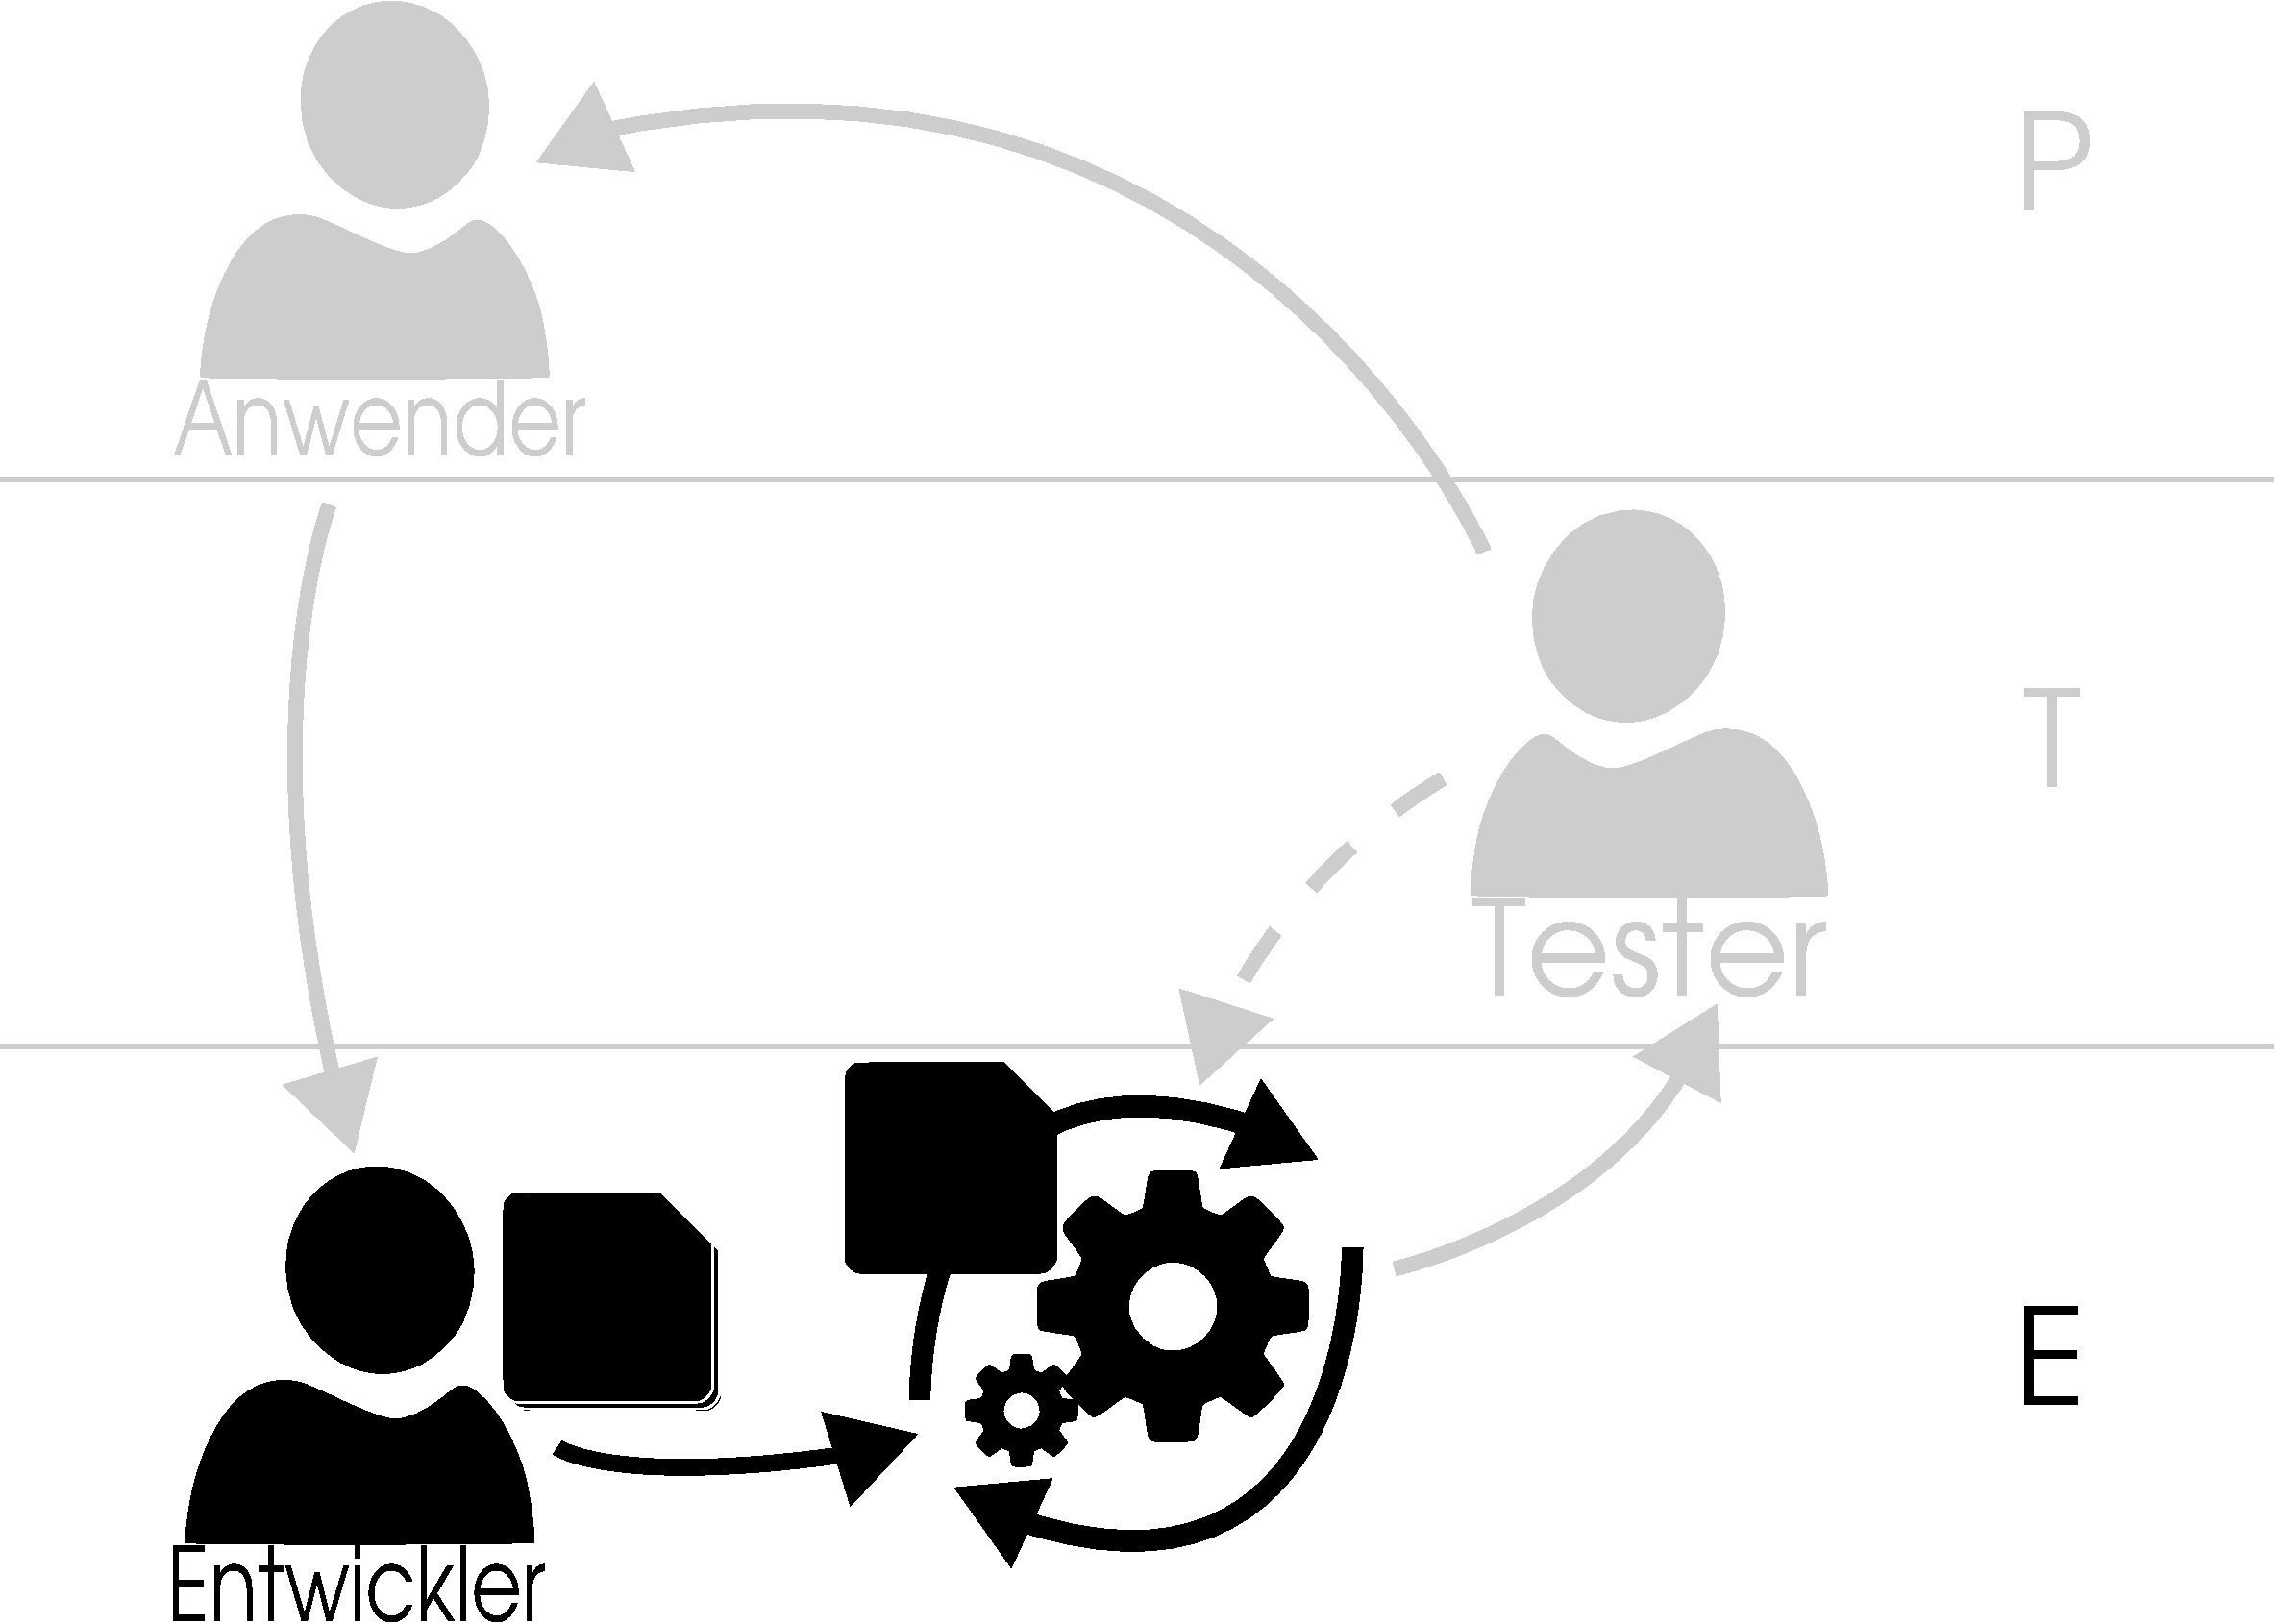
\includegraphics[width=\textwidth]{FDD2}<handout:0>}
  \only<3>{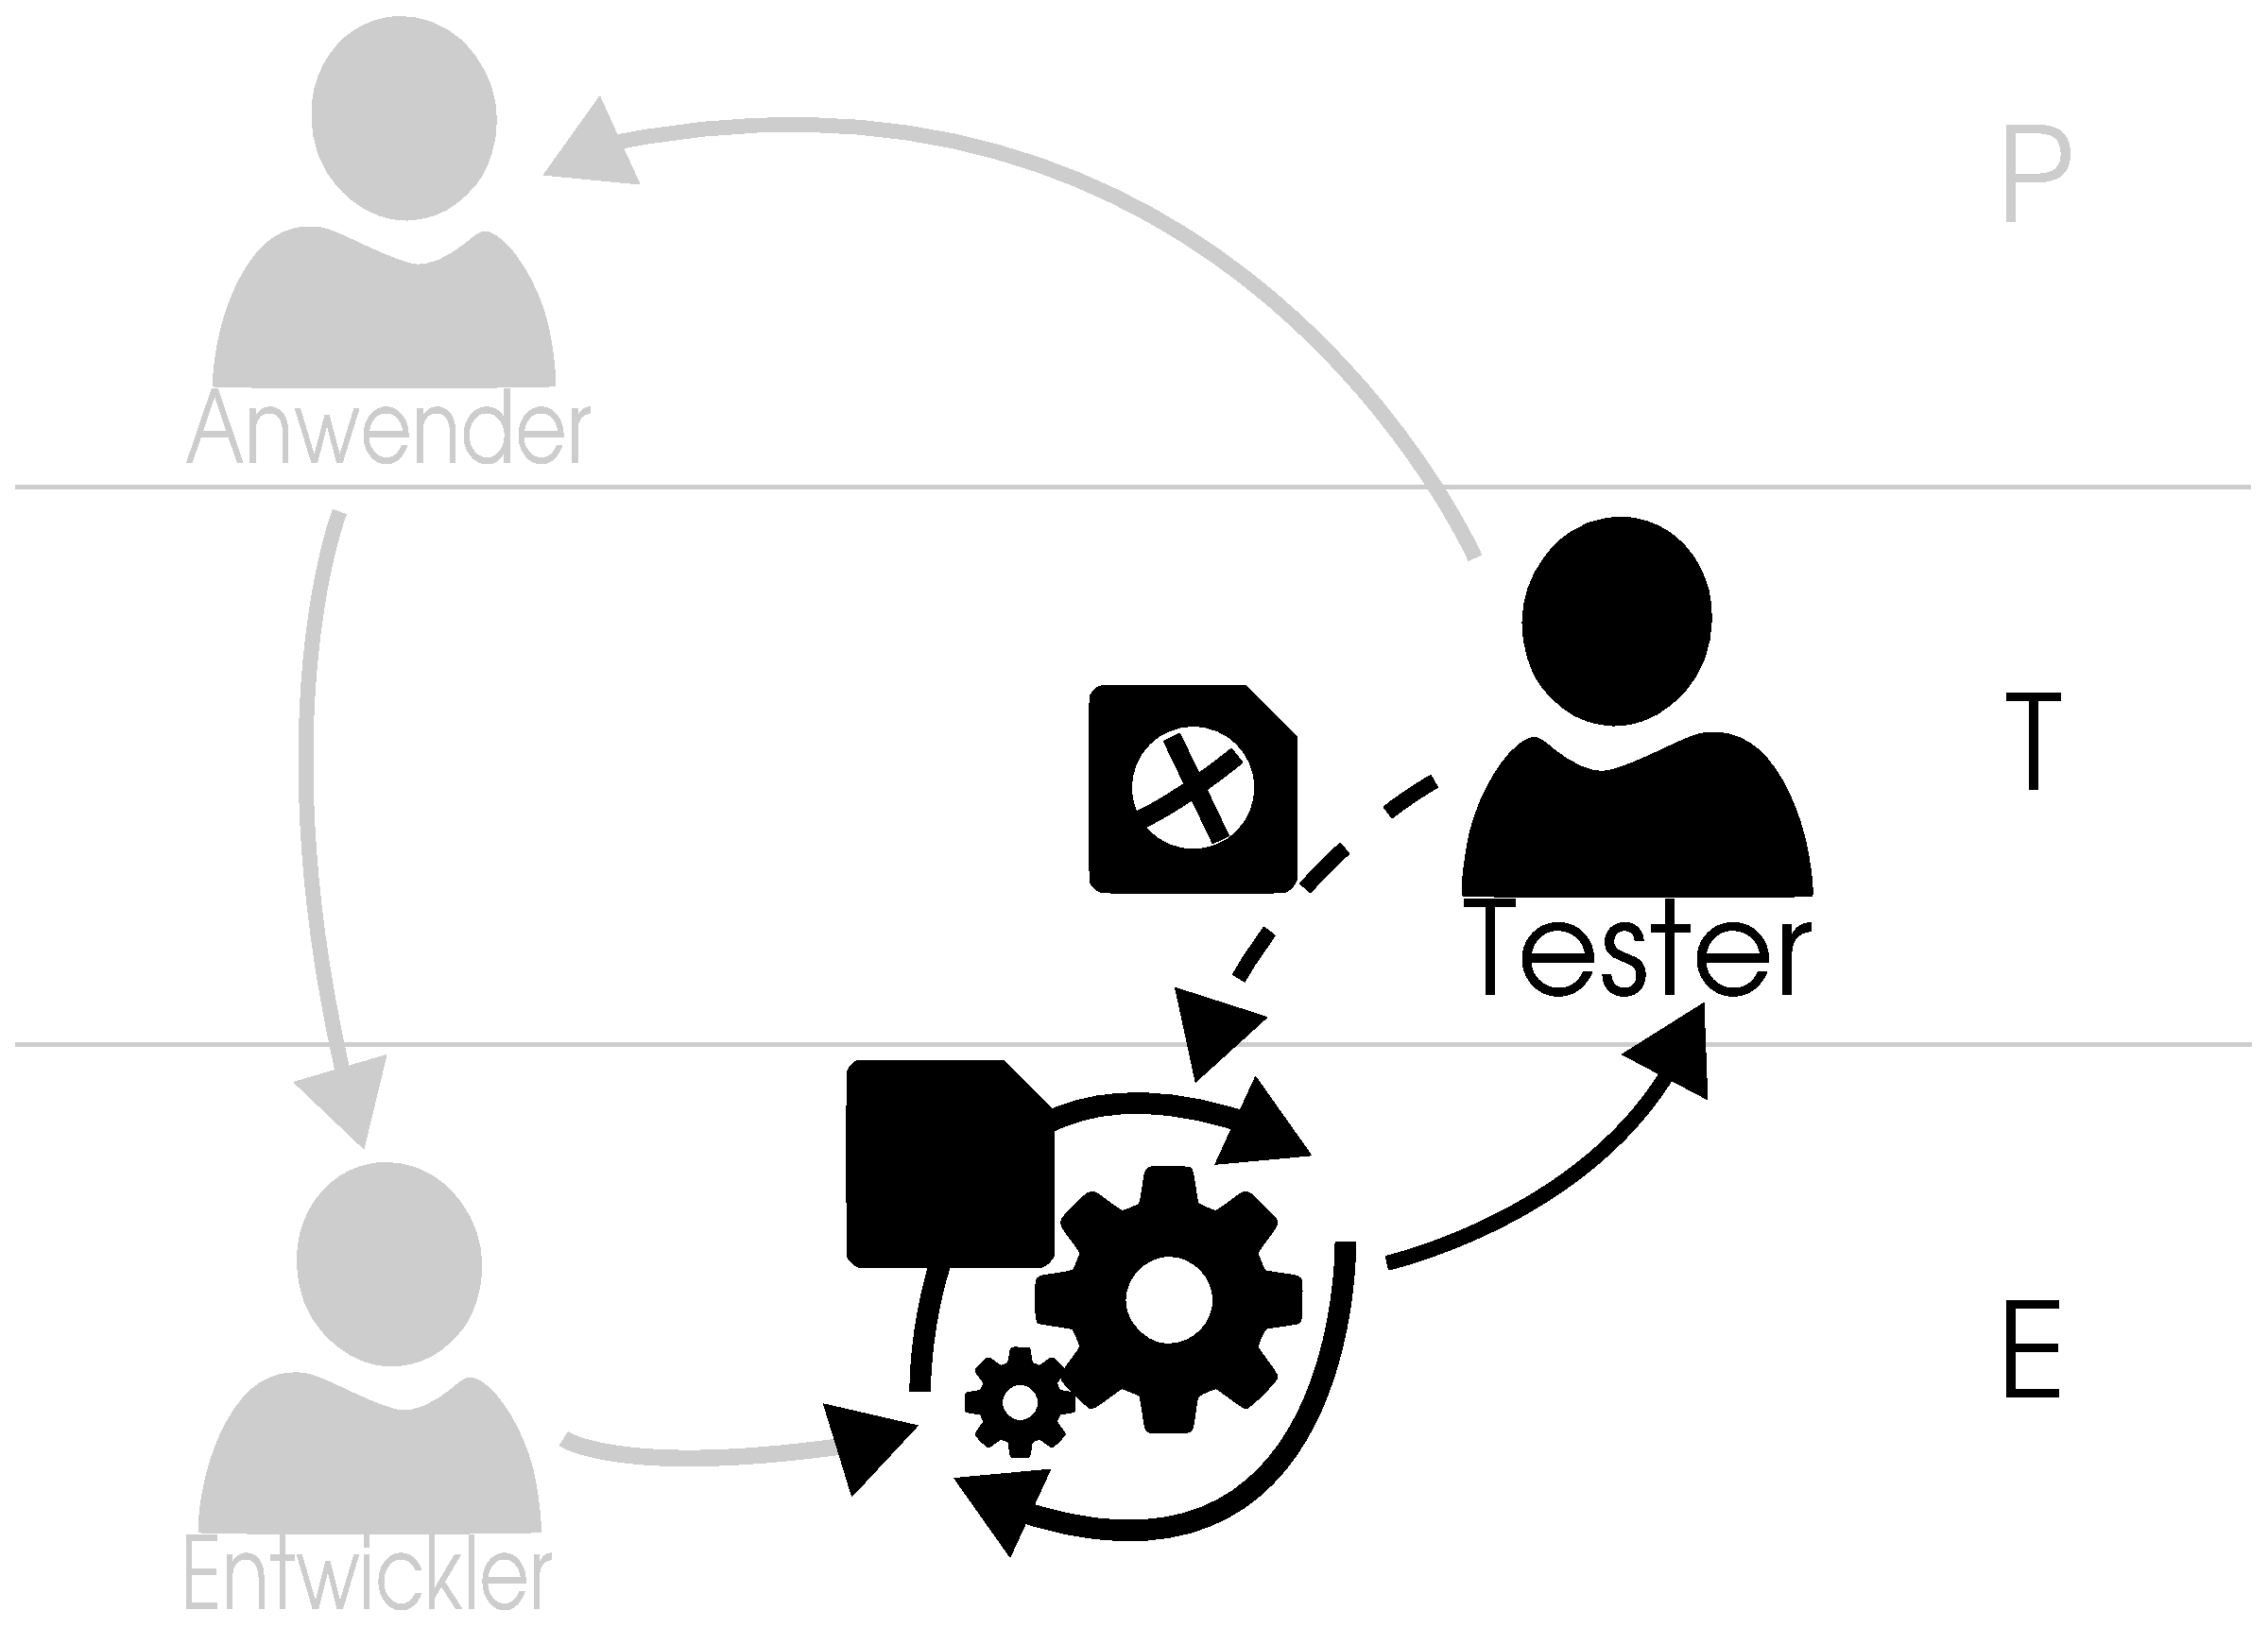
\includegraphics[width=\textwidth]{FDD3}<handout:0>}
  \only<4>{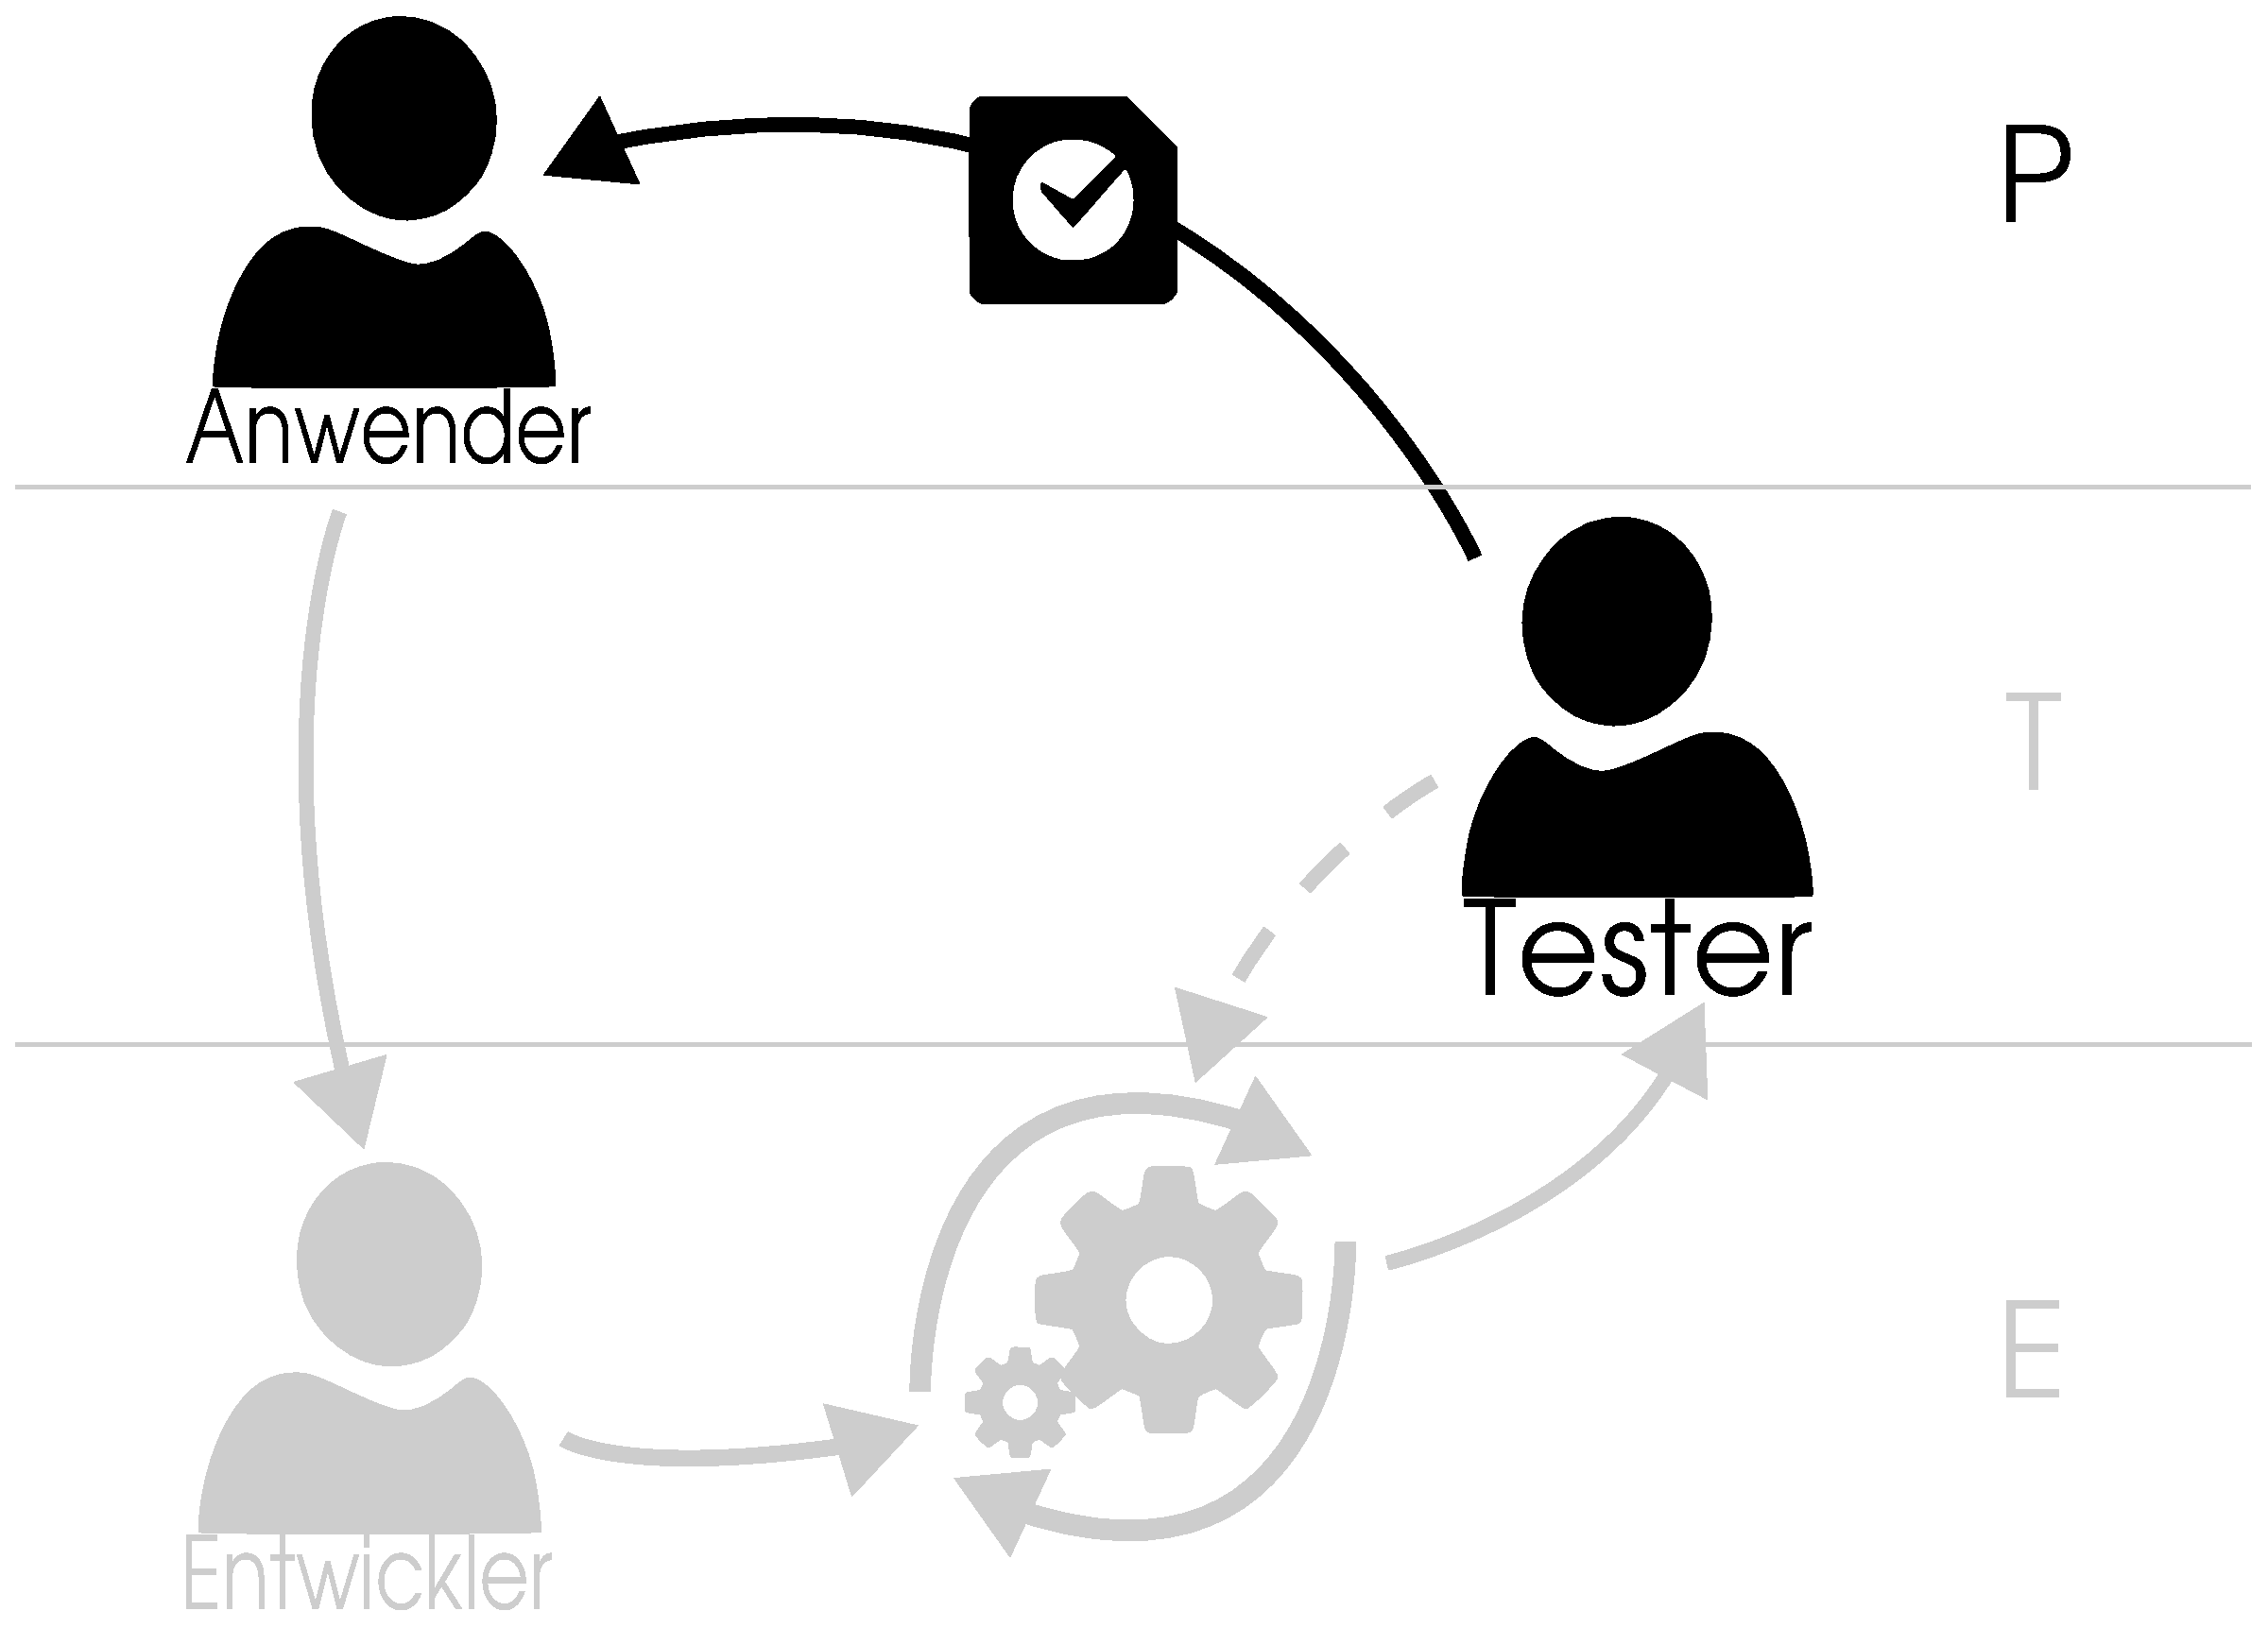
\includegraphics[width=\textwidth]{FDD4}<handout:0>}
  \only<5>{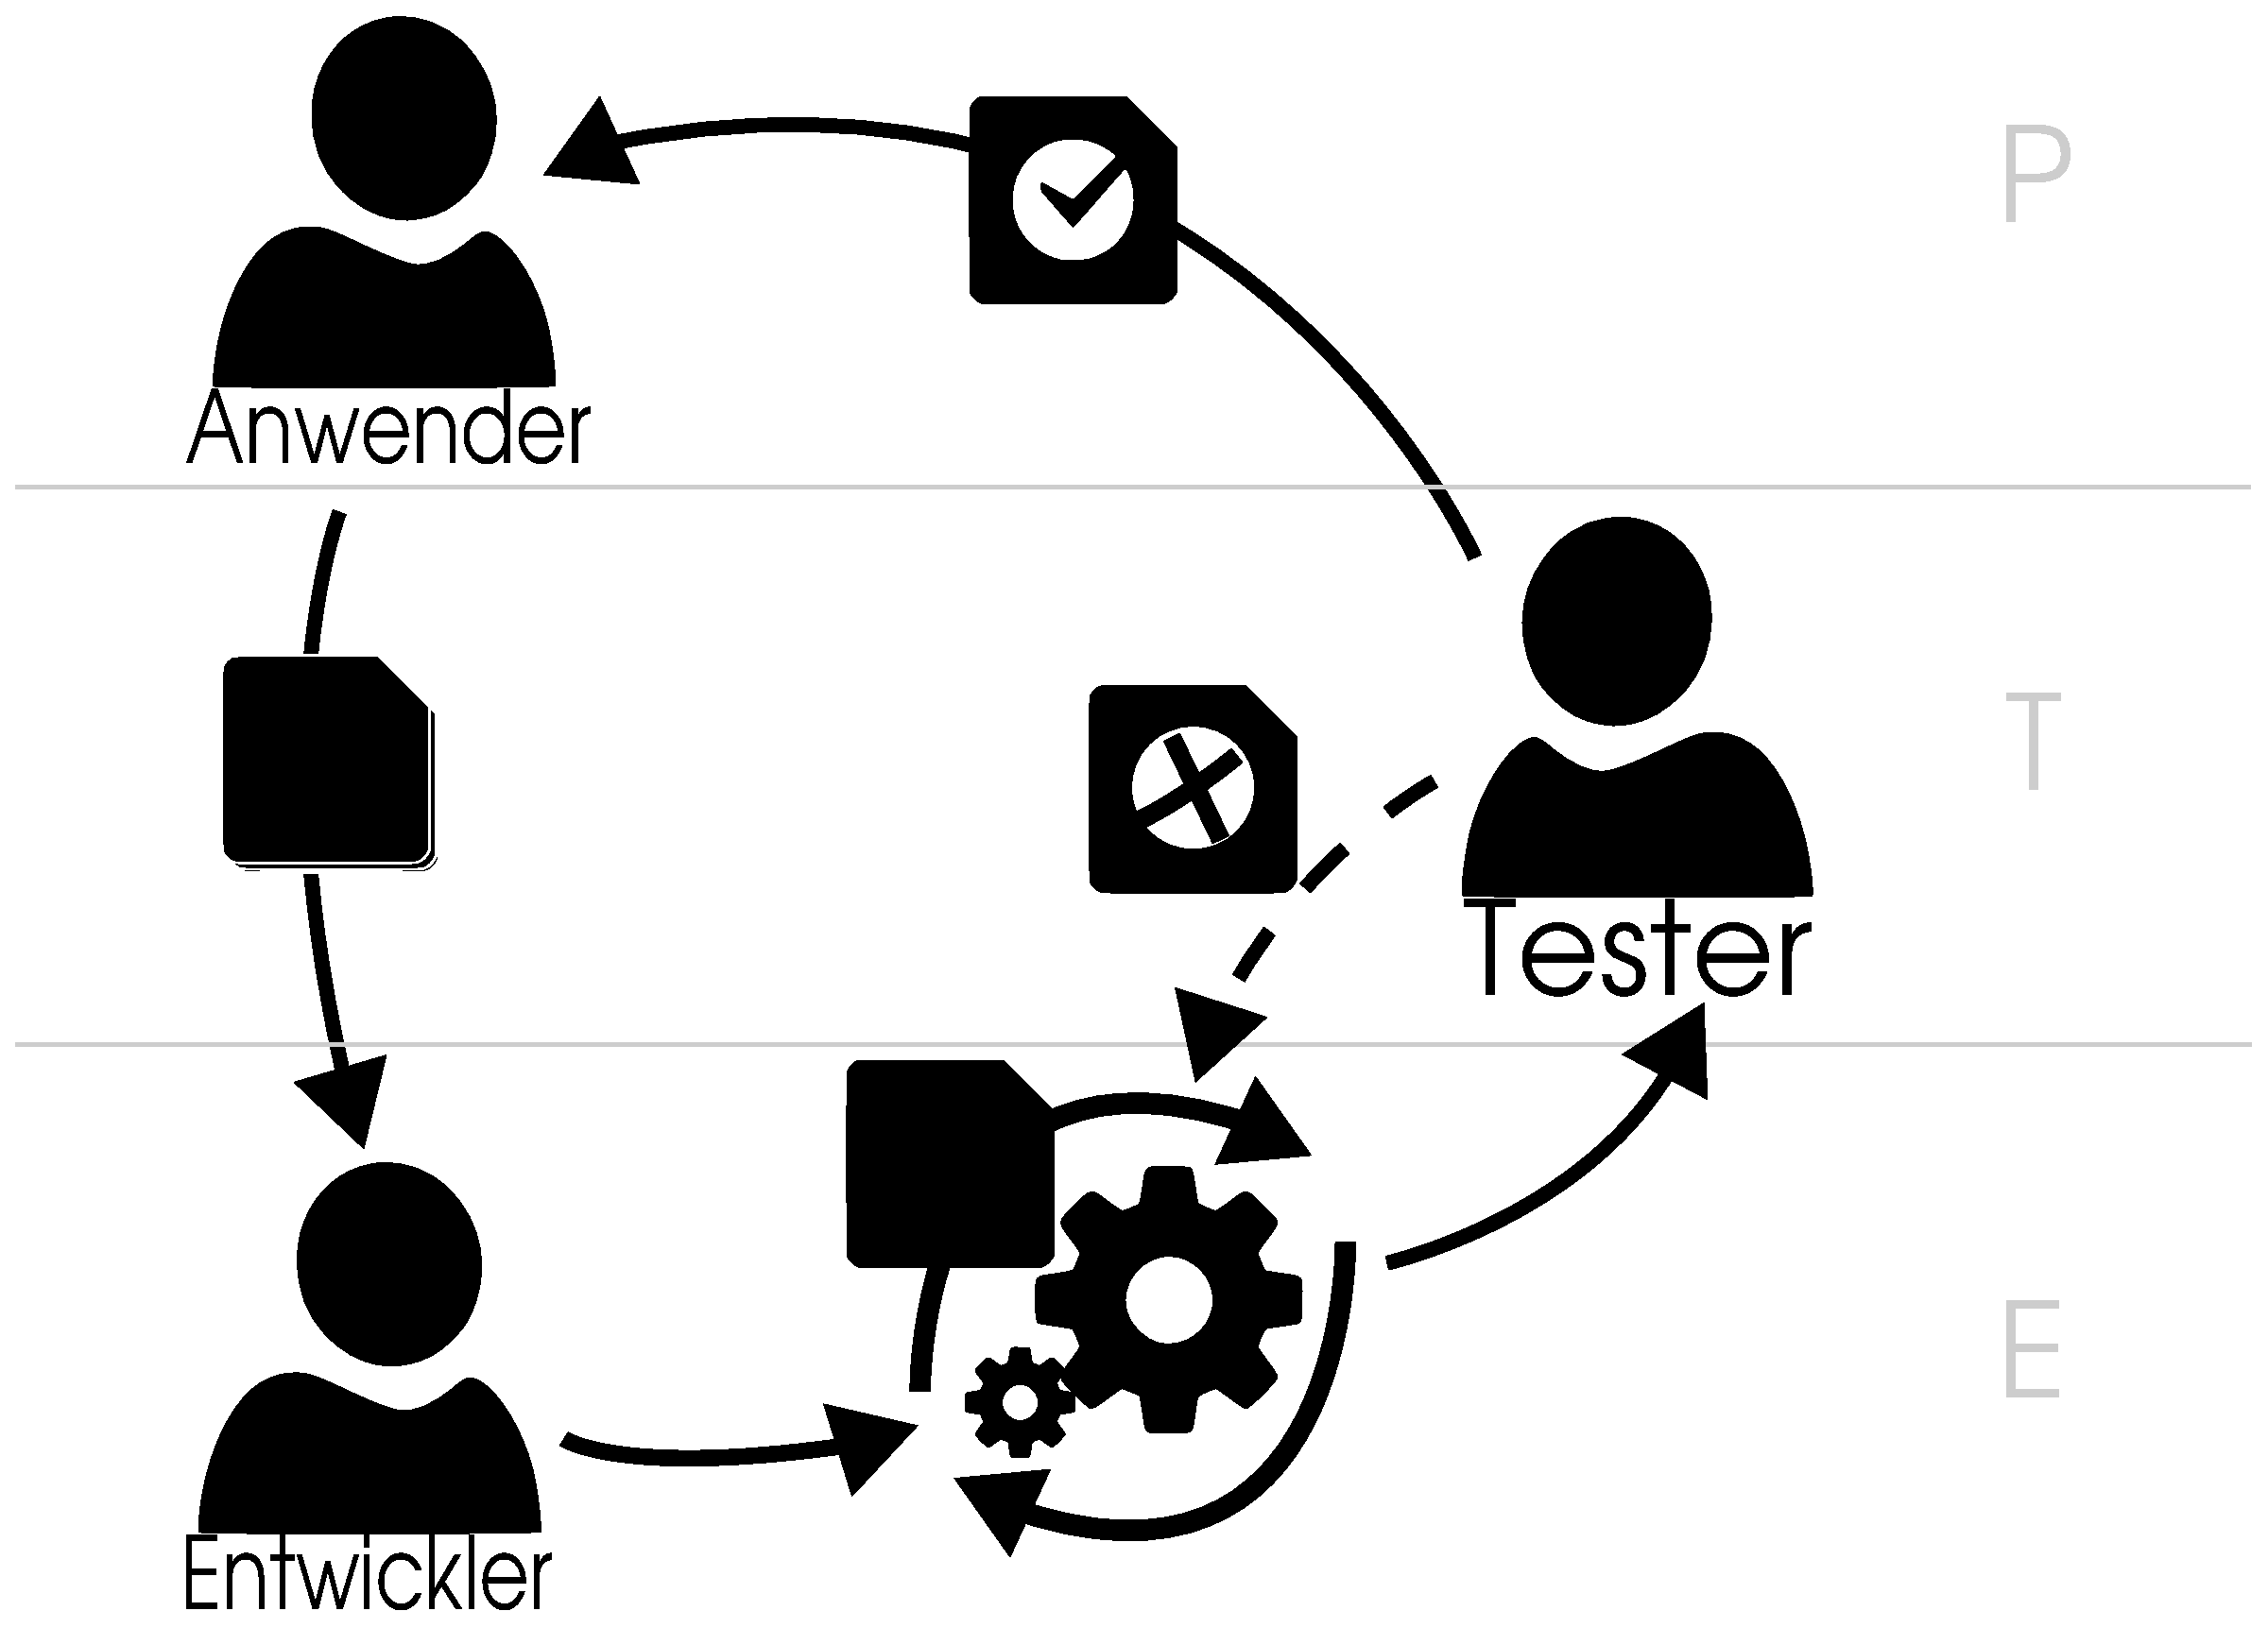
\includegraphics[width=\textwidth]{FDD5}}
 \end{overlayarea}
\end{frame}
\begin{frame}{Komponenten}
\begin{figure}[tb]
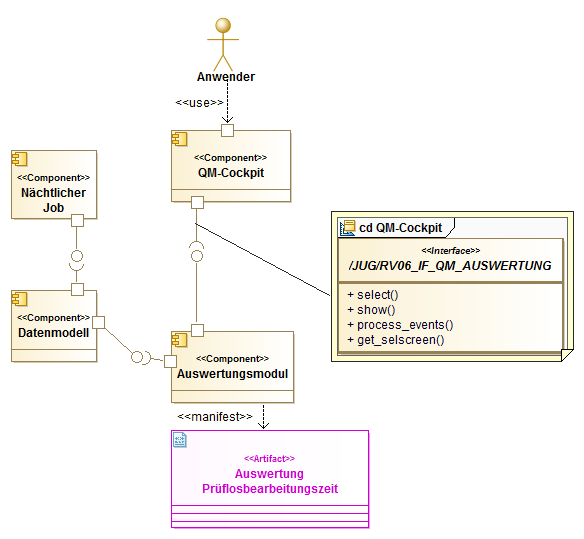
\includegraphics[width=.9\textwidth]{Komponenten}
\end{figure}
\end{frame}
\begin{frame}{Aufbau QM-Cockpit}
 \vspace{3ex}
 \begin{overlayarea}{\textwidth}{.67\textheight}
  \only<1>{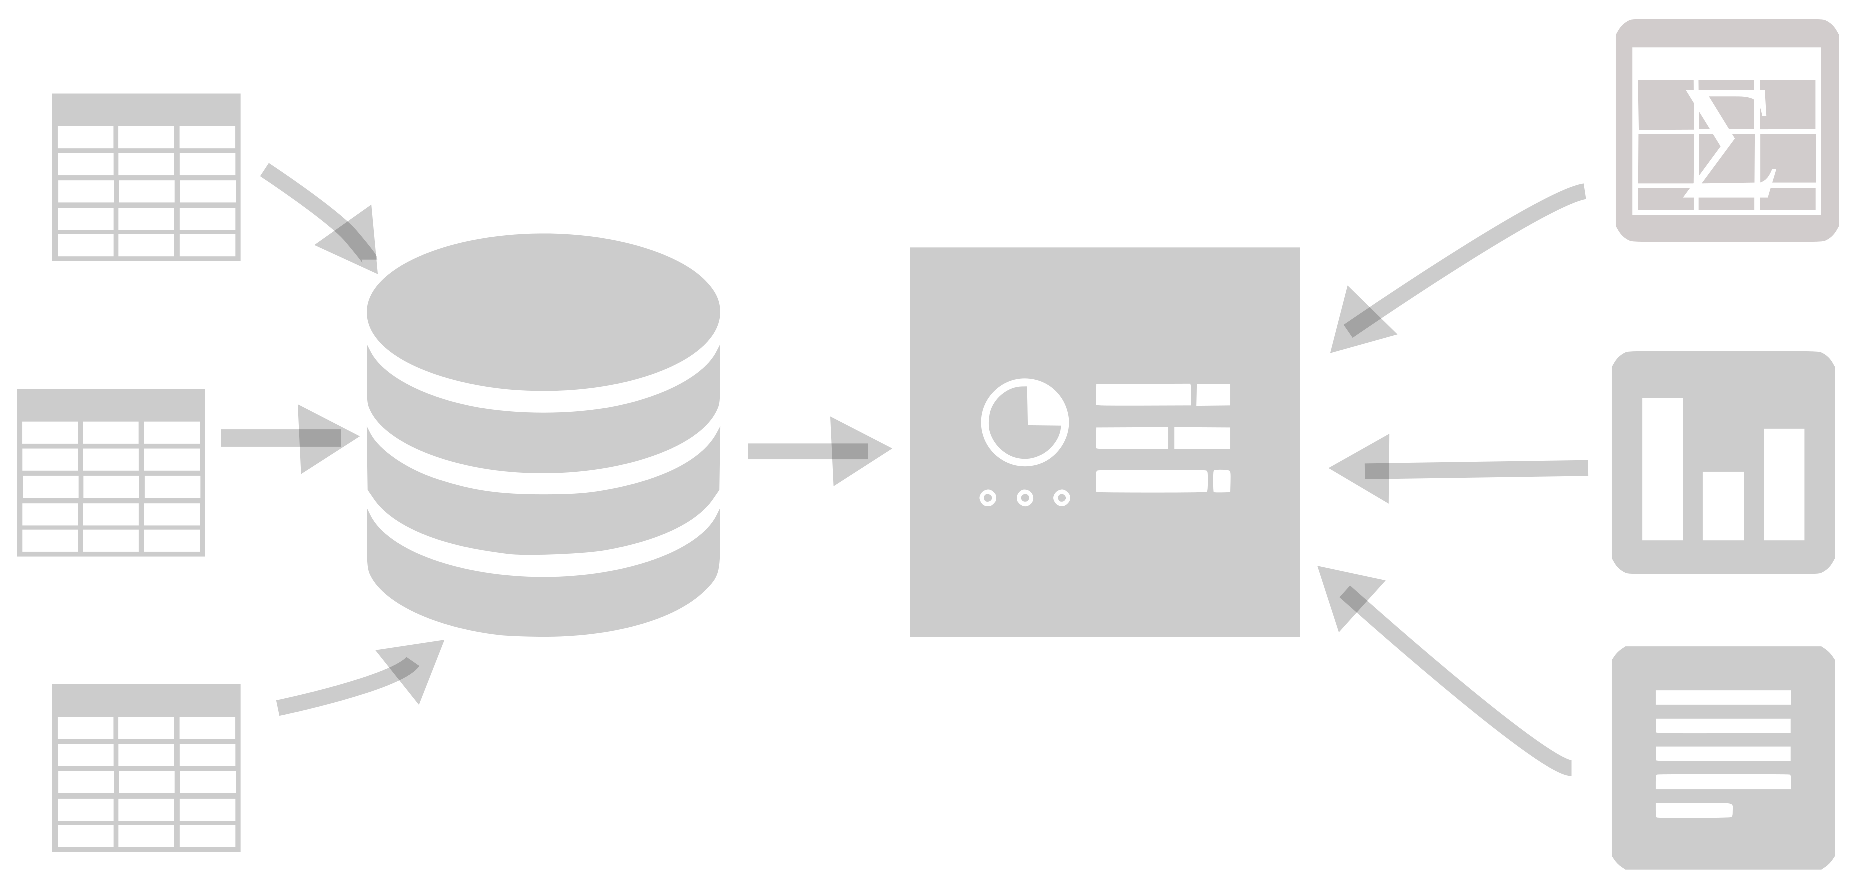
\includegraphics[width=\textwidth]{MVP0}<handout:0>}
  \only<2>{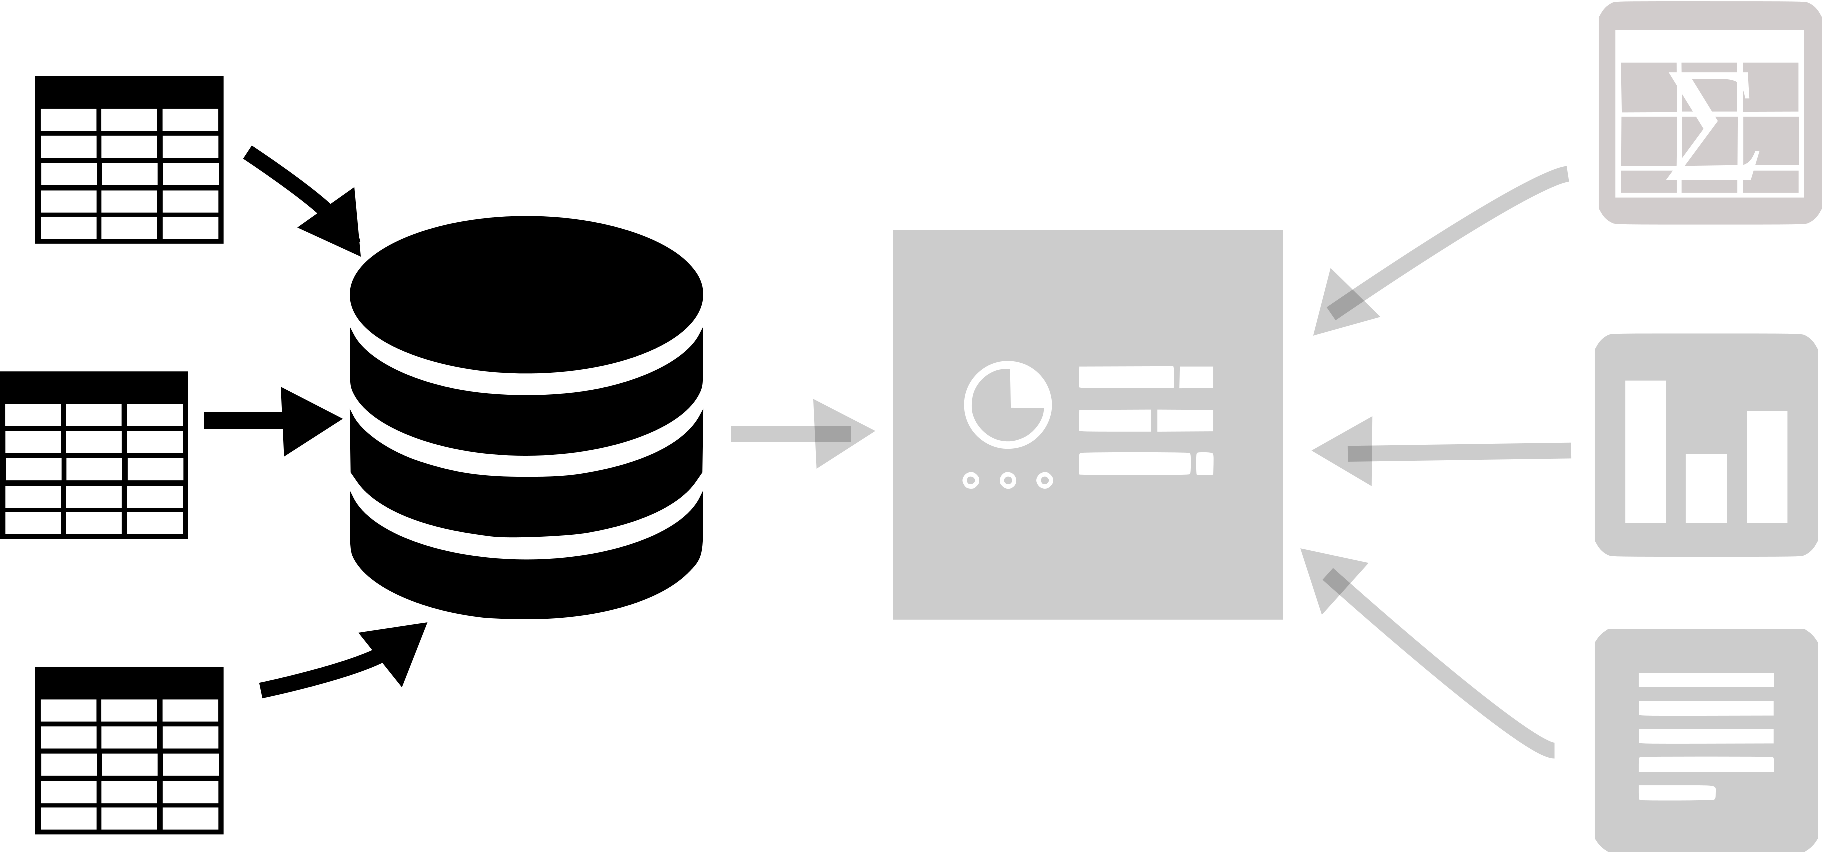
\includegraphics[width=\textwidth]{MVP1}<handout:0>}
  \only<3>{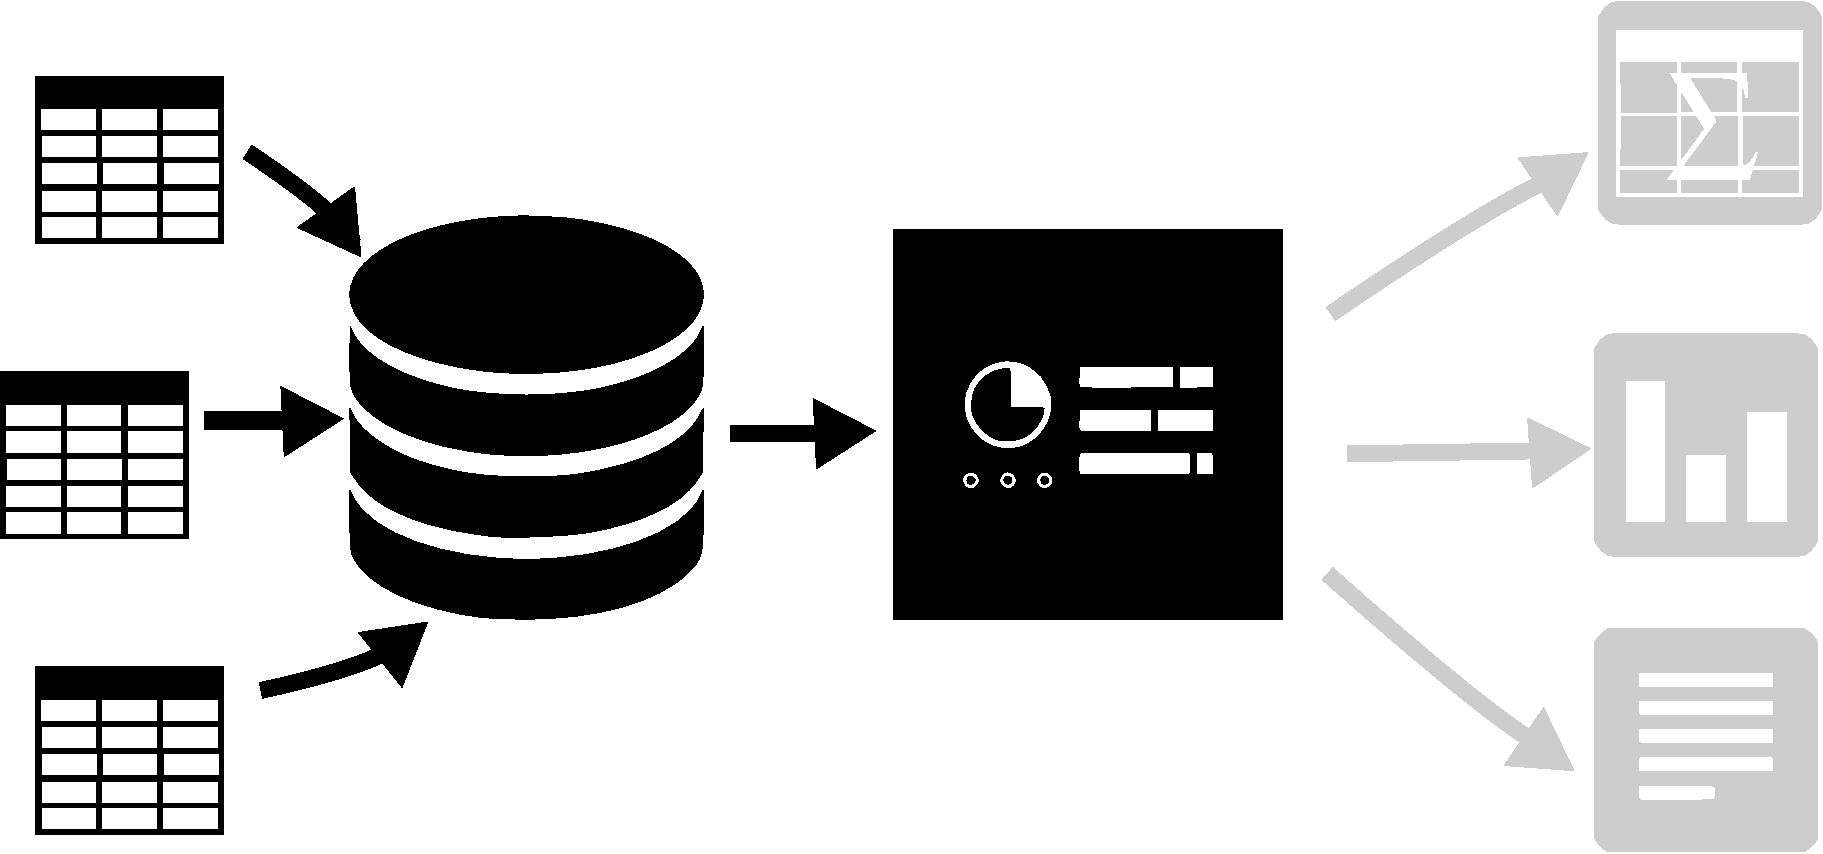
\includegraphics[width=\textwidth]{MVP2}<handout:0>}
  \only<4>{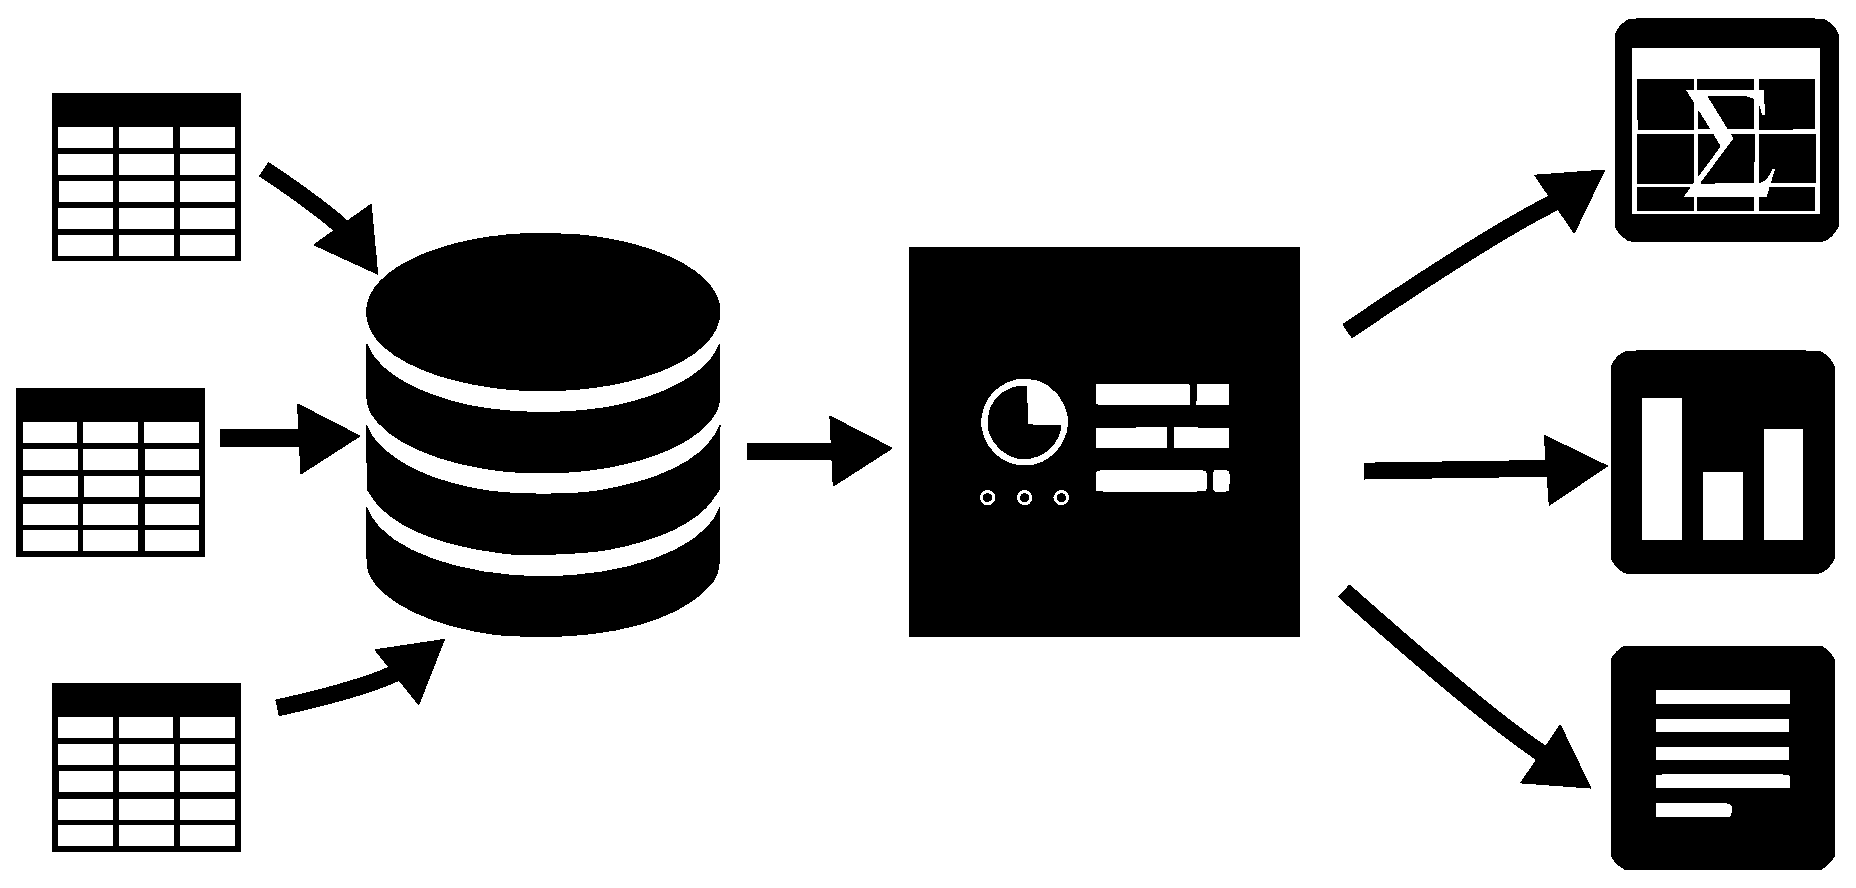
\includegraphics[width=\textwidth]{MVP3}<handout:0>}
  \only<5>{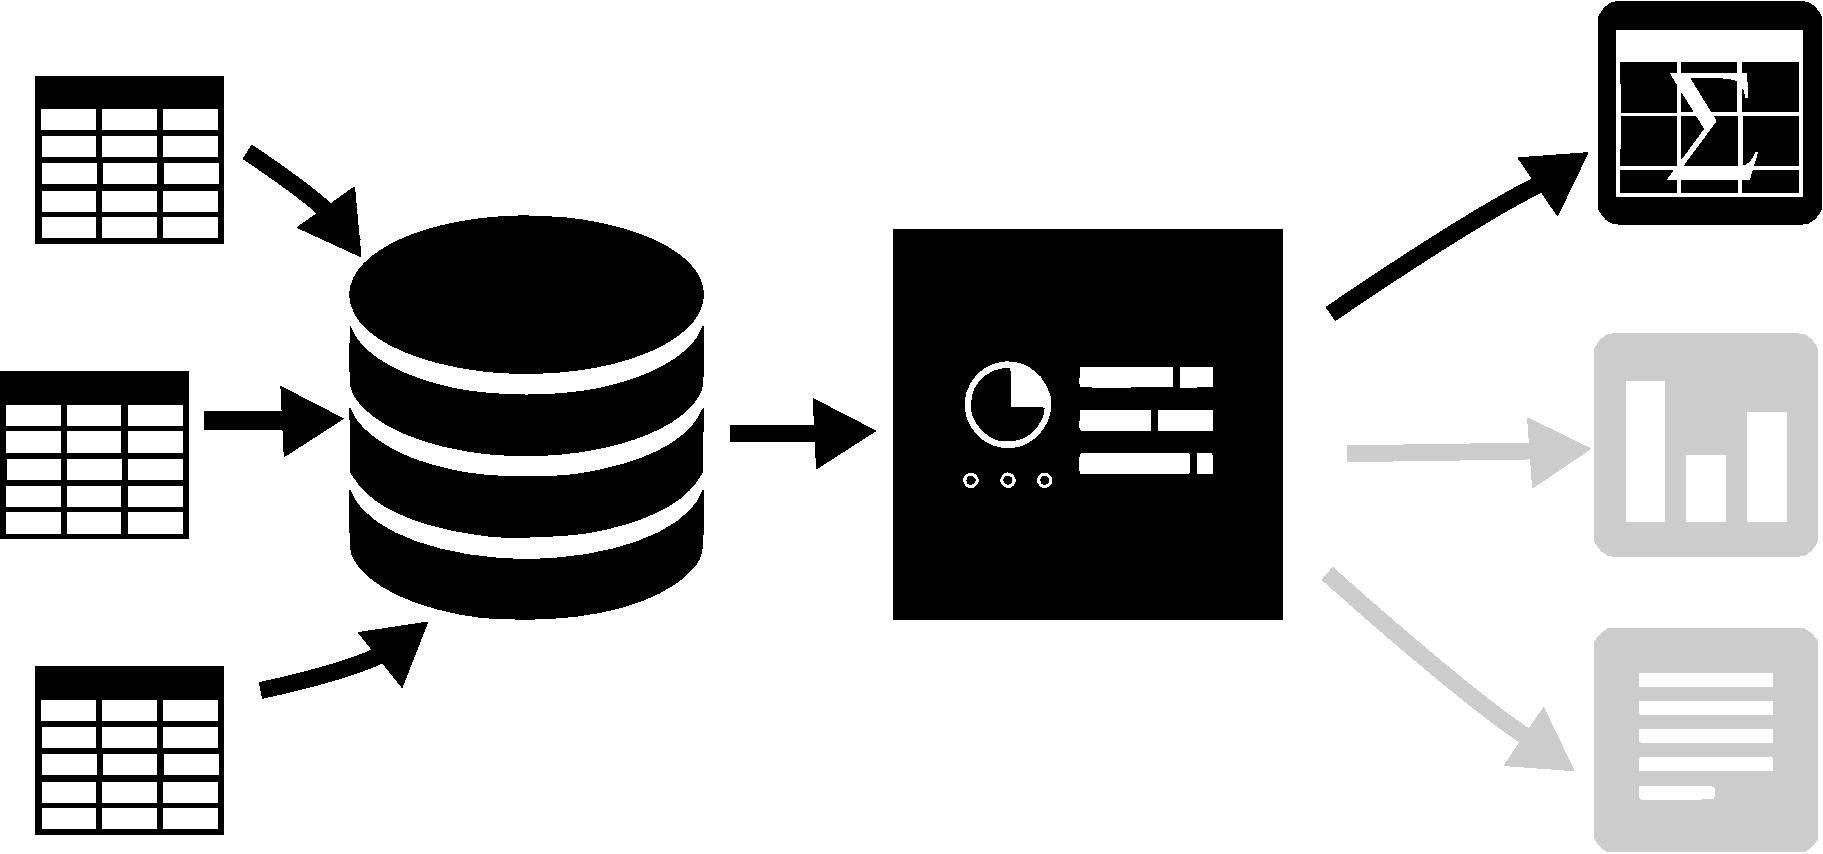
\includegraphics[width=\textwidth]{MVP4}}
 \end{overlayarea}
 \begin{block}{\onslide<2->\textbf<2>{Model} \onslide<3->\textbf<3>{View} \onslide<4->\textbf<4>{Presenter}}\end{block}
\end{frame}
\begin{frame}{QM-Cockpit}
	\huge{TODO} %Cockpit
	            %Auswertungsmodul
\end{frame}

\section{Projektergebnis}
\subsection{Soll-Ist-Vergleich}
\begin{frame}{Projektergebnis}
 \begin{overlayarea}{\textwidth}{.67\textheight}
   \vspace{3ex}
	\begin{figure}[b]
	\only<2>{
\includegraphics[height=.48\textwidth]{Uhr}}
	\only<3>{
\includegraphics[height=.48\textwidth]{Kreisdiagramm}}
	\only<4>{
\includegraphics[height=.36\textwidth]{Strichliste}}
	\only<5>{\huge{TODO!}}
	\end{figure}
 \end{overlayarea}
 
 \begin{overlayarea}{\textwidth}{.33\textheight}
 \centering
 \only<2>{
	{\huge{69\,h Entwicklungszeit}}
 }
 \only<3>{
	{\huge{86\,\% Zeitersparnis}}
 }
 \only<4>{
	{\huge{Vorher}}
 }
 \only<5>{
	{\huge{Nachher}}
 }
 \end{overlayarea}

\end{frame}
\subsection{Fazit}
\begin{frame}[<+->]{Fazit}
\begin{block}{Anf"angliche Bef"urchtung}
\begin{itemize}
\item{Anforderung zu komplex}
\item{Zeit zu knapp}
\end{itemize}
\end{block}
\begin{block}{Aufgetretene Probleme}
\begin{itemize}
\item{zu starke Konkretisierung}
\item{Dokumentation $\Leftrightarrow$ Implementierung}
\end{itemize}
\end{block}
\begin{block}{gewonnene Erkenntnisse}
\begin{itemize}
\item{Top-Down-Prinzip}
\item{Iterative Vorgehensweise}
\end{itemize}
\end{block}
\end{frame}

\begin{frame}{}
\begin{center}
\huge{Vielen Dank f"ur Ihre\\Aufmerksamkeit}\\
\begin{figure}[b!]
\includegraphics{images/platform11b}
\end{figure}
\end{center}
\end{frame}

\end{document}

